\chapter{Planificación}
En la figura \ref{fig:edt} se puede observar el EDT que ha sido seguido para la
realización de este proyecto. Se ha estimado la realización del proyecto en un
plazo inicial de 2 años, comenzando en Octubre, 2014 y finalizando en Octubre de
2016; se han distribuido las tareas como puede observarse en el diagrama de
Gantt ilustrado en la Figura \ref{fig:gantt}. Para el desarrollo de cada
producto se sigue una metodología de desarrollo iterativa e incremental. Al
final de cada iteración se genera un producto intermedio, con las
características acordadas durante el que funcione correctamente con el resto de
productos.  A continuación se detallan las fases principales del proyecto:
\begin{itemize}
	\item T1 - Análisis de requisitos: recolección y análisis de requisitos.
	Organización de requisitos funcionales y no funcionales.

	\item T2 - Desarrollo de la Nube de conductores: incluye todas las actividades
	para el	desarrollo de la aplicación de conductores que será desplegada en la
	nube.

	\item T3 - Desarrollo de la aplicación de ciclistas: actividades para el
	desarrollo 	de la aplicación de ciclistas y el casco \gls{ble}.

	\item T4 - Desarrollo de las aplicaciones vehiculares: actividades para el
	desarrollo de la \gls{rsu}, \gls{obu} y \glossary{hmi}.

	\item T5 - Validación: pruebas que se han desarrollado en la calle para
	validar diferentes partes del proyecto, y grabación de una demo del
	funcionamiento del proyecto completo.

	\item T6 - Estudios adjuntos: estudios realizados para el desarrollo de
	diferentes áreas del proyecto.
\end{itemize}

\begin{figure}[t]
	\begin{center}
		\rotatebox{90} {
			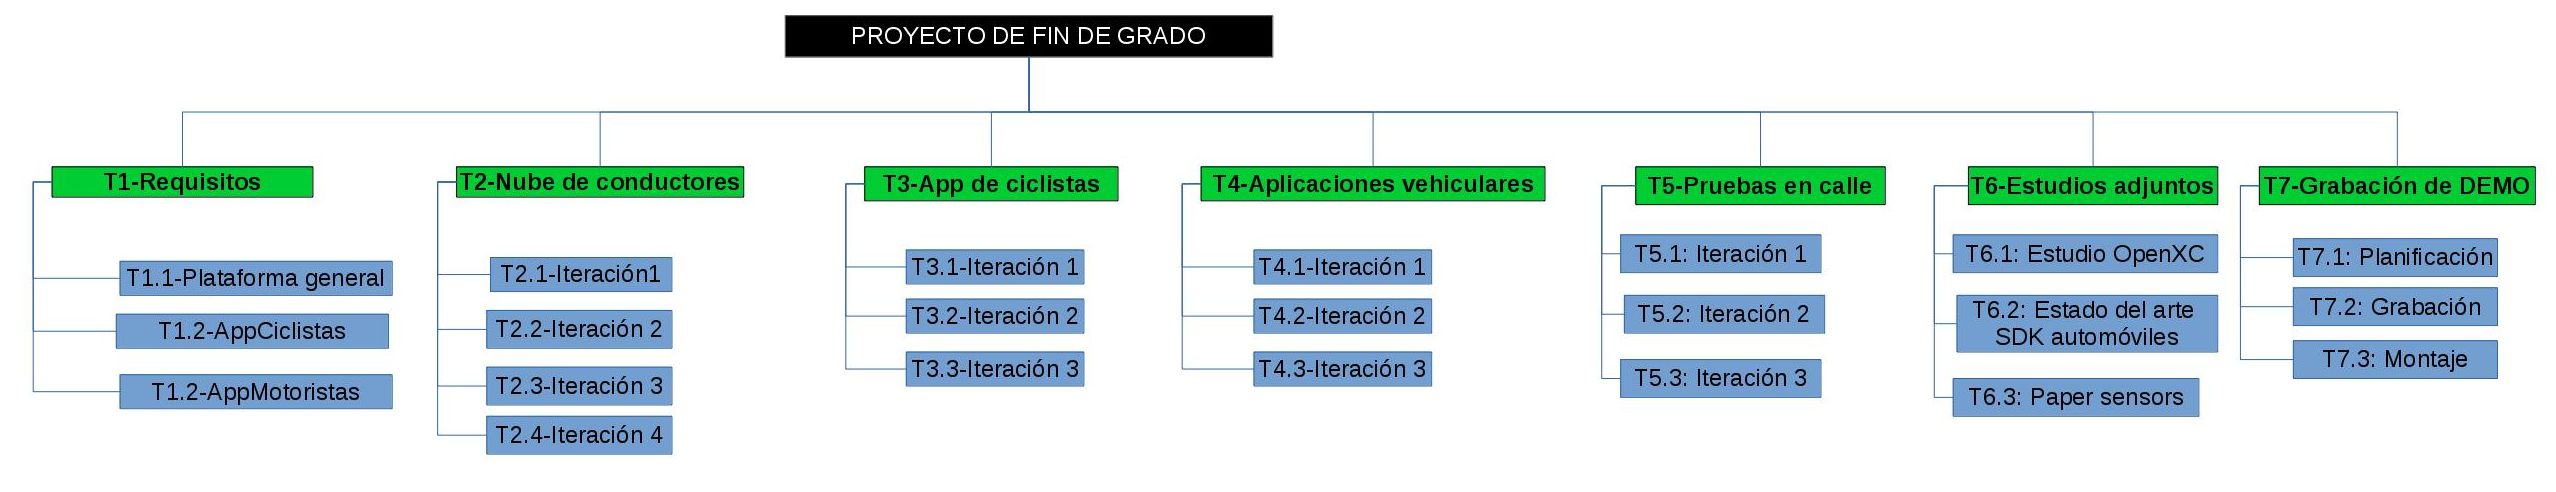
\includegraphics[scale=0.35]{EDT}
		}
		\caption{Diagrama de desglose de trabajo}
		\label{fig:edt}
	\end{center}
\end{figure}

\begin{figure}[t]
	\rotatebox{90} {
		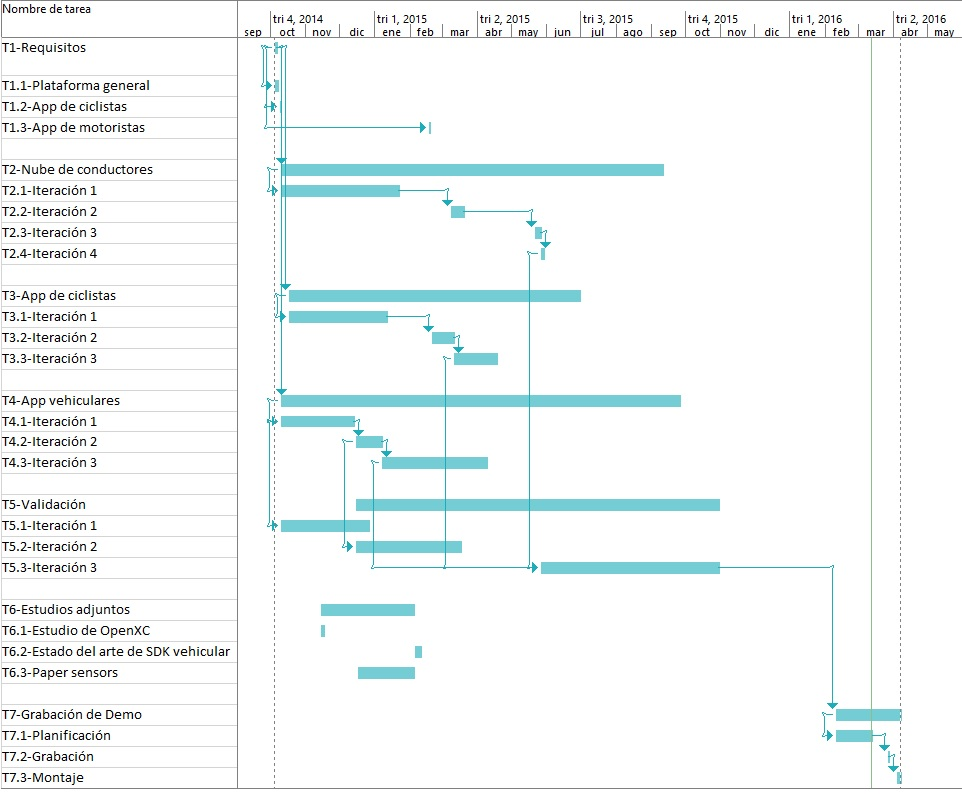
\includegraphics[scale=0.6]{DiagramaGantt}
	}
	\caption{Diagrama de Gantt}
	\label{fig:gantt}
\end{figure}

Las iteraciones se realizan dentro de las tareas T2, T3 y T4. En cada uno del
las iteraciones se realiza cada una de las siguientes actividades:
\begin{itemize}
	\item Diseño: selección de las especificaciones a implementar y realización
	del diseño de las funciones a implementar en la aplicación.

	\item Desarrollo y depuración: desarrollo y depuración de las funciones
	diseñadas.

	\item Documentación: generación de la documentación de toda la fase
	(comentarios en código, documentos explicativos, prototipos generados...).
\end{itemize}
\FloatBarrier
\section{Paquetes de trabajo}
\begin{table}[ht]
	\centering
	\caption{T1 - Análisis de requisitos}
	\begin{tabular}{ll}
		\toprule
		\multicolumn{2}{c}{\textbf{T1 - Análisis de requisitos}} \\
		\midrule
		\textbf{Duración} & 4 días \\
		\midrule
		\textbf{Objetivos} &
		\begin{tabular}{p{0.8\textwidth}}
			Recolección y análisis de requisitos. Organización de requisitos
			funcionales y no funcionales.
		\end{tabular} \\
		\midrule
		\textbf{Descripción} &
		 \begin{tabular}{p{0.8\textwidth}}
		 	\begin{itemize}
		 		\item Iteración 1: implementación de la arquitectura básica,base de
				datos y acceso a través de sockets.

		 		\item Iteración 2: mejora del formato de mensajes utilizado en la
				comunicación, cambio del acceso por sockets a servlets, e inclusión de
				algoritmos de predicción de accidentes.

		 		\item Iteración 3: cambiada la comunicación con la aplicación de
				ciclistas a \gls{gcm}.

		 		\item Iteración 4: optimización de la plataforma.
		 	\end{itemize}
		 \end{tabular} \\
		\bottomrule
	\end{tabular}
\end{table}

\begin{table}[ht]
	\centering
	\caption{T2 - Desarrollo de la Nube de conductores}
	\begin{tabular}{ll}
		\toprule
		\multicolumn{2}{c}{\textbf{T2 - Desarrollo de la Nube de conductores}} \\
		\midrule
		\textbf{Duración} & 102 días \\
		\midrule
		\textbf{Objetivos} &
		\begin{tabular}{p{0.8\textwidth}}
			Diseño, desarrollo, depuración y despliegue en la nube de la aplicación
			''Nube de conductores''.
		\end{tabular} \\
		\midrule
		\textbf{Descripción} &
		\begin{tabular}{p{0.8\textwidth}}
			\begin{itemize}
				\item Iteración 1: implementación de la arquitectura básica,
				base de datos y acceso a través de sockets.

				\item Iteración 2: mejora del formato de mensajes utilizado en la
				comunicación, cambio del acceso por sockets a servlets, e inclusión de
				algoritmos de predicción de accidentes.

				\item Iteración 3: cambiada la comunicación con la aplicación de
				ciclistas a \gls{gcm}.

				\item Iteración 4: optimización de la plataforma.
			\end{itemize}
		\end{tabular} \\
		\bottomrule
	\end{tabular}
\end{table}

\begin{table}[ht]
	\centering
	\caption{T3 - Desarrollo de la aplicación de ciclistas}
	\begin{tabular}{ll}
		\toprule
		\multicolumn{2}{c}{\textbf{T3 - Desarrollo de la aplicación de ciclistas}}\\
		\midrule
		\textbf{Duración} & 94 días \\
		\midrule
		\textbf{Objetivos} &
		\begin{tabular}{p{0.8\textwidth}}
			Diseño, desarrollo, depuración de la aplicación para ciclistas y el casco
			de seguridad \gls{ble}.
		\end{tabular} \\
		\midrule
		\textbf{Descripción} &
		\begin{tabular}{p{0.8\textwidth}}
			\begin{itemize}
				\item Iteración 1: desarrollo de la base de la aplicación; incluye
				salidas individuales y en grupo.

				\item Iteración 2: mejora de la sensibilidad del \gls{gps}, prueba con
				mensajes \gls{udp} en salidas en grupo, cambio de comunicación a la nube
				a través de mensajes \Gls{http/1.1} y soporte a versiones antiguas de
				Android.

				\item Iteración 3: empleo de \gls{gcm} para la recepción de mensajes y
				desarrollo del casco \gls{ble}.
			\end{itemize}
		\end{tabular} \\
		\bottomrule
	\end{tabular}
\end{table}

\begin{table}[ht]
	\centering
	\caption{T4 - Desarrollo de las aplicaciones vehiculares}
	\begin{tabular}{ll}
		\toprule
		\multicolumn{2}{c}{\textbf{T4 - Desarrollo de las aplicaciones vehiculares}}\\
		\midrule
		\textbf{Duración} & 65 días \\
		\midrule
		\textbf{Objetivos} &
		\begin{tabular}{p{0.8\textwidth}}
			Diseño, desarrollo, depuración y despliegue de las tres aplicaciones para
			vehículos: \gls{obu}, \gls{rsu} y \gls{hmi}.
		\end{tabular} \\
		\midrule
		\textbf{Descripción} &
		\begin{tabular}{p{0.8\textwidth}}
			\begin{itemize}
				\item Iteración 1: base de las aplicaciones \gls{obu} y \gls{rsu}.

				\item Iteración 2: cambio de comunicación a servlets y mejora de los
				mensajes empleados en la comunicación.

				\item Iteración 3: optimización de la plataforma e implementación de la
				aplicación para el \gls{hmi}.
			\end{itemize}
		\end{tabular} \\
		\bottomrule
	\end{tabular}
\end{table}

\begin{table}[ht]
	\centering
	\caption{T5 - Validación}
	\begin{tabular}{ll}
		\toprule
		\multicolumn{2}{c}{\textbf{T5 - Validación}} \\
		\midrule
		\textbf{Duración} & 94 días \\
		\midrule
		\textbf{Objetivos} &
		\begin{tabular}{p{0.8\textwidth}}
			Durante cada iteración de la validación se desarrollan tres actividades:
			una primera para planificar qué pruebas se desean hacer y qué datos se
			desean obtener, así como preparar la aplicación para pruebas. Durante la
			segunda actividad se desarrollan las pruebas. Y finalmente, la tercera
			actividad, se recogen y estudian los resultados y se proponen mejoras
			para futuros desarrollos. Para realizar las estadísticas de los datos
			obtenidos durante las pruebas se ha empleado la librería \emph{matplotlib}
			de \emph{Python}.
		\end{tabular} \\
		\midrule
		\textbf{Descripción} &
		\begin{tabular}{p{0.8\textwidth}}
			\begin{itemize}
				\item Iteración 1: pruebas de rendimiento en comunicaciones \gls{v2x}.

				\item Iteración 2: comunicación \gls{v2v} en entornos urbanos.

				\item Iteración 3: prueba del sistema completo.

				\item Grabación de la demo:
				\begin{itemize}
					\item Planificación: Requisitos generales para la grabación:
					selección de personas que ayuden durante el rodaje, selección de
					escenas y escenarios, materiales, fechas...

					\item Grabación.

					\item Montaje: montaje del vídeo y post-producción.
				\end{itemize}
			\end{itemize}
		\end{tabular} \\
		\bottomrule
	\end{tabular}
\end{table}

\begin{table}[th]
	\centering
	\caption{T6 - Estudios adjuntos}
	\begin{tabular}{ll}
		\toprule
		\multicolumn{2}{c}{\textbf{T6 - Estudios adjuntos}} \\
		\midrule
		\textbf{Duración} & 32 días \\
		\midrule
		\textbf{Objetivos} &
		\begin{tabular}{p{0.8\textwidth}}
			Documentar los estudios realizados durante el desarrollo de las diferentes
			áreas del proyecto para ser publicadas o para facilitar futuros
			desarrollos.
		\end{tabular} \\
		\midrule
		\textbf{Descripción} &
		\begin{tabular}{p{0.8\textwidth}}
			\begin{itemize}
			\item Estudio de OpenXC: se desarrolla un estudio sobre la plataforma
			OpenXC y la posibilidad de su uso en el proyecto.

			\item Estado del arte de Unificación de SDK: se estudia la creación de un
			subproyecto para	desarrollar aplicaciones en el \gls{hmi} de los
			vehículos en	diferentes plataformas; AndroidAuto, CarPlay...

			\item Paper para sensors: desarrollo de un artículo para MDPI sobre
			comunicaciones vehiculares y su uso sobre \gls{vru}.
			\end{itemize}
		\end{tabular} \\
		\bottomrule
	\end{tabular}
\end{table}

\FloatBarrier
\chapter{Descripción de la realización}\label{cha:descripcion_realizacion}
En el capítulo \ref{cha:alcance} se puede observar el EDT que ha sido seguido para
la realización de este proyecto. Para el desarrollo de cada producto se sigue una
metodología de desarrollo iterativa e incremental. Al final de cada iteración se
genera un producto intermedio, con las características acordadas durante el que
funcione correctamente con el resto de productos.  A continuación se detallan las
fases principales del proyecto:
\begin{itemize}
	\item \textbf{T1 - Requisitos}: recolección y análisis de requisitos. Organización
	de requisitos funcionales y no funcionales.

	\item \textbf{T2 - Nube de conductores}: incluye todas las actividades para el
	desarrollo de la aplicación de conductores que será desplegada en la nube.

	\item \textbf{T3 - App de ciclistas}: actividades para el desarrollo de la
	aplicación de ciclistas y el casco \gls{ble}.

	\item \textbf{T4 - Aplicaciones vehiculares}: actividades para el desarrollo
	de la \gls{rsu}, \gls{obu} y \glossary{hmi}.

	\item \textbf{T5 - Pruebas en la calle}: pruebas que se han desarrollado en la
	calle para validar diferentes partes del proyecto.

	\item \textbf{T6 - Grabación de DEMO}: grabación de una demo del funcionamiento del
	proyecto completo.

	\item \textbf{T7 - Estudios adjuntos}: estudios realizados para el desarrollo de
	diferentes áreas del proyecto.
\end{itemize}

Las iteraciones se realizan dentro de las tareas T2, T3 y T4. En cada uno del las
iteraciones se realiza cada una de las siguientes actividades:
\begin{itemize}
	\item \textbf{Diseño}: selección de las especificaciones a implementar y realización
	del diseño de las funciones a implementar en la aplicación.

	\item \textbf{Desarrollo y depuración}: desarrollo y depuración de las funciones
	diseñadas.

	\item \textbf{Documentación}: generación de la documentación de toda la fase
	(comentarios en código, documentos explicativos, prototipos generados...).
\end{itemize}


La estrategia seguida durante el proyecto puede observarse en la imagen \ref{fig:estrategia}.
Inicialmente se reúnen los requisitos necesarios y se realiza un diseño de las funcionalidades
a incluir, se producen varias iteraciones hasta que todos los requisitos son satisfechos. Una
vez finalizado el diseño se pasa al desarrollo, el cual incluye depuración y pruebas unitarias.
Cuando el desarrollo ha finalizado correctamente, se pueden añadir nuevos requisitos o pasar
a pruebas en calle si han sido programadas con anterioridad; algunas pruebas requieren de
adaptar parte del programa al carácter de las pruebas. Una vez finalizadas las pruebas, si se
han descubierto fallos en el software, es reparado y si se decide que es requerido ampliar
la plataforma se vuelve a iniciar el ciclo.
\begin{figure}[H]
	\begin{center}
		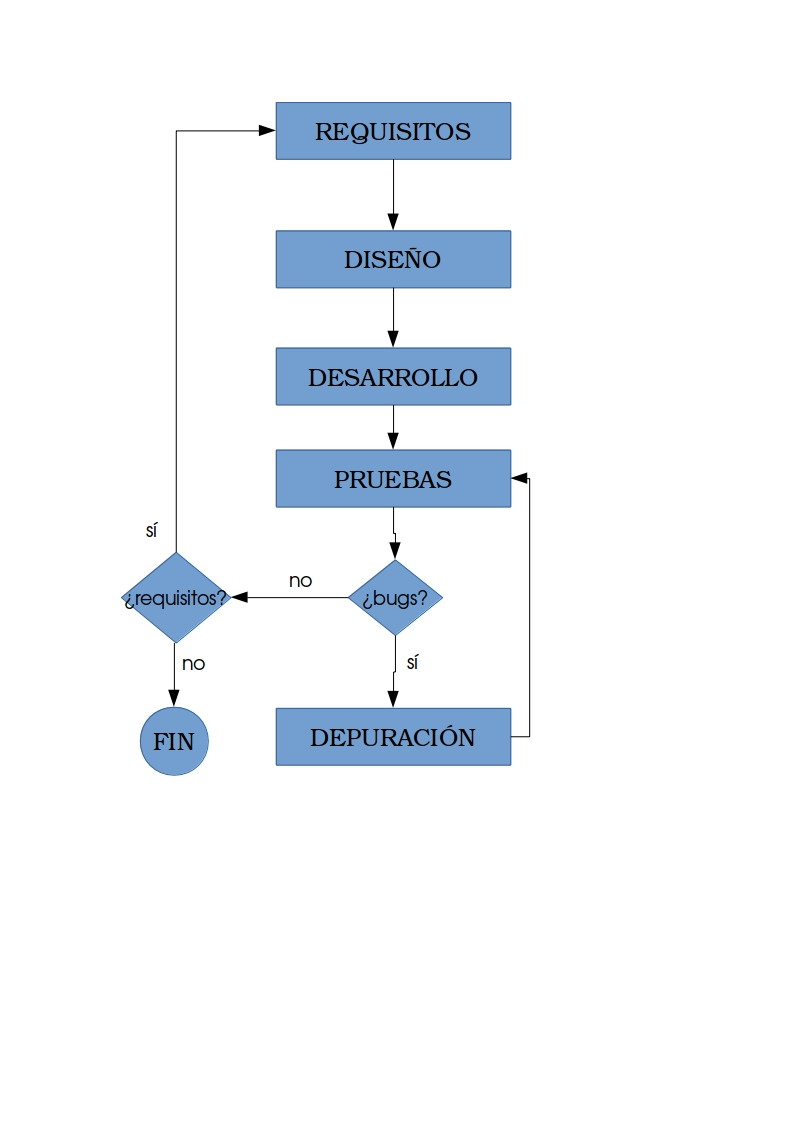
\includegraphics[scale=0.4]{diagrama-estrategia}
		\caption{Estrategia del desarrollo}
		\label{fig:estrategia}
	\end{center}
\end{figure}

Se ha estimado la realización del proyecto en un plazo inicial de 2 años, comenzando en Octubre, 2014 y
finalizando en Octubre de 2016. En la figura \ref{fig:EDT} se muestra la división inicial de las actividades
del proyecto.
\begin{figure}[H]
	\begin{center}
		\rotatebox{90} {
			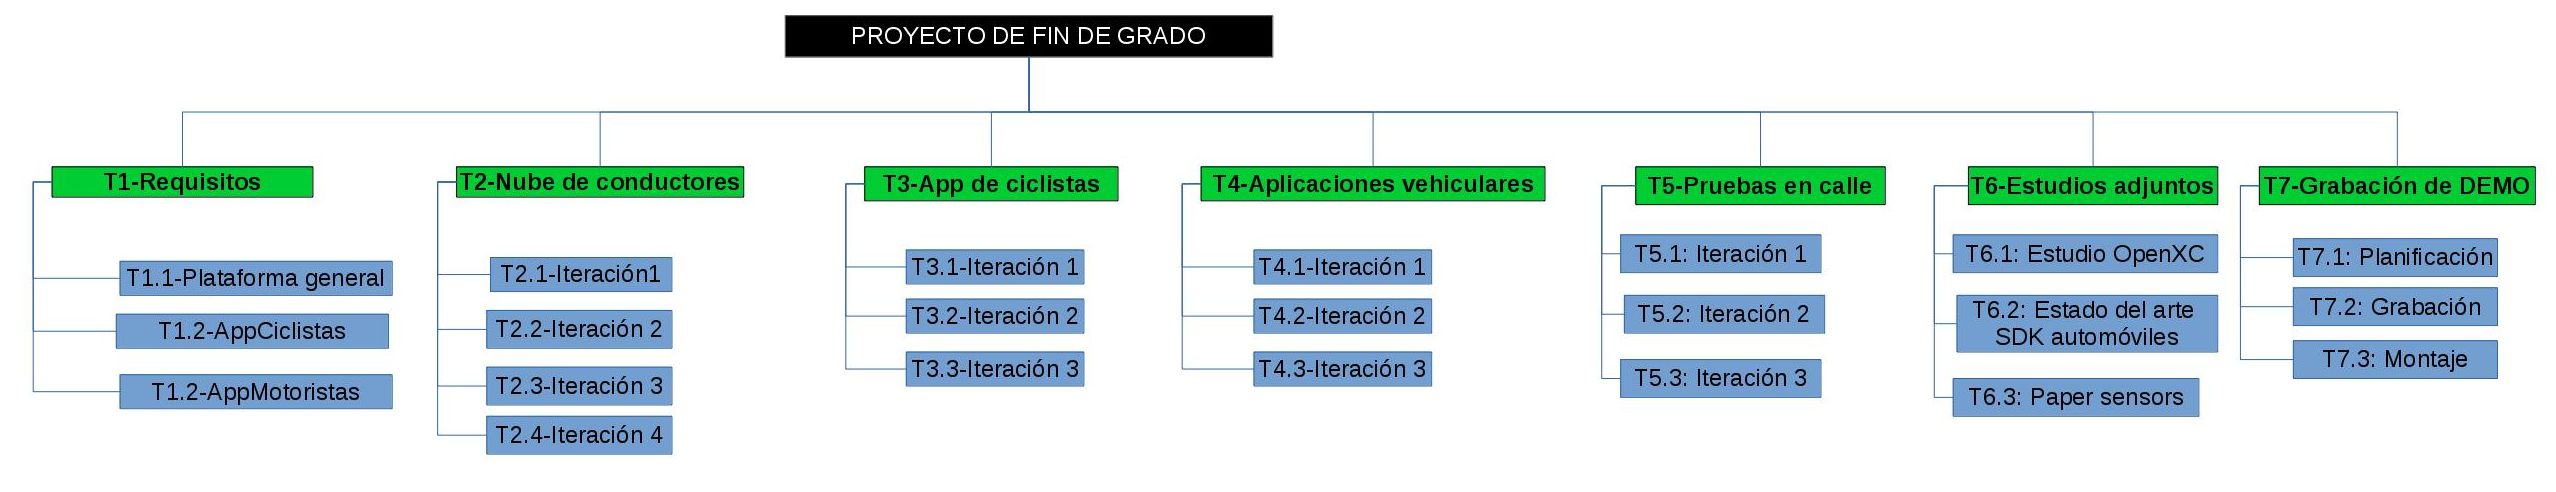
\includegraphics[scale=0.25]{EDT}
		}
		\caption{Diagrama de desglose de trabajo}
		\label{fig:EDT}
	\end{center}
\end{figure}

\section{Tareas}
\subsection{T1 - Requisitos}
\begin{itemize}
	\item \textbf{Plataforma general}: requisitos de la aplicación en la nube
	y las aplicaciones vehiculares básicas (\gls{obu} y \gls{rsu}).

	\item \textbf{AppCiclistas:} requisitos de la aplicación para los ciclistas
	y el casco BLE.

	\item \textbf{AppMotoristas:} requisitos de la aplicación para el \gls{hmi} de
	los vehículos.
\end{itemize}

\subsection{T2 - Nube de conductores}
\begin{itemize}
	\item \textbf{Iteración 1:} implementación de la arquitectura básica, base de
	datos y acceso a través de sockets.

	\item \textbf{Iteración 2:} mejora del formato de mensajes utilizado en la
	comunicación, cambio del acceso por	sockets a servlets, e inclusión de
	algoritmos de predicción de accidentes.

	\item \textbf{Iteración 3:} cambiada la comunicación con la aplicación de
	ciclistas a \gls{gcm}.

	\item \textbf{Iteración 4:} optimización de la plataforma.
\end{itemize}

\subsection{T3 - App de ciclistas}
\begin{itemize}
	\item \textbf{Iteración 1:} desarrollo de la base de la aplicación; incluye
	salidas individuales y en grupo.

	\item \textbf{Iteración 2:} mejora de la sensibilidad del GPS, prueba con
	mensajes UDP en salidas en grupo, cambio de comunicación a la nube a través
	de mensajes \Gls{http/1.1} y soporte a versiones antiguas de Android.

	\item \textbf{Iteración 3:} empleo de \gls{gcm} para la recepción de mensajes
	y desarrollo del casco \gls{ble}.
\end{itemize}

\subsection{T4 - Aplicaciones vehiculares}
\begin{itemize}
	\item \textbf{Iteración 1:} base de las aplicaciones \gls{obu} y \gls{rsu}.

	\item \textbf{Iteración 2:} cambio de comunicación a servlets y mejora de
	los mensajes empleados en la comunicación.

	\item \textbf{Iteración 3:} optimización de la plataforma e implementación
	de la aplicación para el \gls{hmi}.
\end{itemize}

\subsection{T5 - Validación}
Durante cada iteración de la validación se desarrollan tres actividades: una
primera para planificar qué pruebas se desean hacer y qué datos se desean obtener,
así como preparar la aplicación para pruebas. Durante la segunda actividad se
desarrollan las pruebas. Y finalmente, la tercera actividad, se recogen y estudian
los resultados y se proponen mejoras para futuros desarrollos. Para realizar las 
estadísticas de los datos obtenidos durante las pruebas se ha empleado la librería
\emph{matplotlib} de \emph{Python}.
\begin{itemize}
	\item \textbf{Iteración 1:} pruebas de rendimiento en comunicaciones \gls{v2x}.

	\item \textbf{Iteración 2:} comunicación \gls{v2v} en entornos urbanos.

	\item \textbf{Iteración 3:} prueba del sistema completo.
\end{itemize}

\subsection{T6 - Estudios adjuntos}
\begin{itemize}
	\item \textbf{Estudio de OpenXC}: se desarrolla un estudio sobre la plataforma
	OpenXC y la posibilidad de su uso en el proyecto.

	\item \textbf{Estado del arte de Unificación de SDK:} se estudia la creación de
	un subproyecto para	desarrollar aplicaciones en el \gls{hmi} de los vehículos en
	diferentes plataformas; AndroidAuto, CarPlay...

	\item \textbf{Paper para sensors}: desarrollo de un artículo para MDPI sobre
	comunicaciones vehiculares y su uso sobre \gls{vru}.
\end{itemize}

\subsection{T7 - Grabación de DEMO}
\begin{itemize}
	\item \textbf{Planificación:} Requisitos generales para la grabación: selección
	de personas que ayuden durante el rodaje, selección de escenas y escenarios,
	materiales, fechas...

	\item \textbf{Grabación}.

	\item \textbf{Montaje}: montaje del vídeo y post-producción.
\end{itemize}

